%% bare_conf.tex
%% V1.4b
%% 2015/08/26
%% by Michael Shell
%% See:
%% http://www.michaelshell.org/
%% for current contact information.
%%
%% This is a skeleton file demonstrating the use of IEEEtran.cls
%% (requires IEEEtran.cls version 1.8b or later) with an IEEE
%% conference paper.
%%
%% Support sites:
%% http://www.michaelshell.org/tex/ieeetran/
%% http://www.ctan.org/pkg/ieeetran
%% and
%% http://www.ieee.org/

%%*************************************************************************
%% Legal Notice:
%% This code is offered as-is without any warranty either expressed or
%% implied; without even the implied warranty of MERCHANTABILITY or
%% FITNESS FOR A PARTICULAR PURPOSE! 
%% User assumes all risk.
%% In no event shall the IEEE or any contributor to this code be liable for
%% any damages or losses, including, but not limited to, incidental,
%% consequential, or any other damages, resulting from the use or misuse
%% of any information contained here.
%%
%% All comments are the opinions of their respective authors and are not
%% necessarily endorsed by the IEEE.
%%
%% This work is distributed under the LaTeX Project Public License (LPPL)
%% ( http://www.latex-project.org/ ) version 1.3, and may be freely used,
%% distributed and modified. A copy of the LPPL, version 1.3, is included
%% in the base LaTeX documentation of all distributions of LaTeX released
%% 2003/12/01 or later.
%% Retain all contribution notices and credits.
%% ** Modified files should be clearly indicated as such, including  **
%% ** renaming them and changing author support contact information. **
%%*************************************************************************


% *** Authors should verify (and, if needed, correct) their LaTeX system  ***
% *** with the testflow diagnostic prior to trusting their LaTeX platform ***
% *** with production work. The IEEE's font choices and paper sizes can   ***
% *** trigger bugs that do not appear when using other class files.       ***                          ***
% The testflow support page is at:
% http://www.michaelshell.org/tex/testflow/

\documentclass[conference]{IEEEtran}
\usepackage[pdftex]{graphicx}
\usepackage{tabularx}
\usepackage{booktabs}

% Some Computer Society conferences also require the compsoc mode option,
% but others use the standard conference format.
%
% If IEEEtran.cls has not been installed into the LaTeX system files,
% manually specify the path to it like:
% \documentclass[conference]{../sty/IEEEtran}





% Some very useful LaTeX packages include:
% (uncomment the ones you want to load)


% *** MISC UTILITY PACKAGES ***
%
%\usepackage{ifpdf}
% Heiko Oberdiek's ifpdf.sty is very useful if you need conditional
% compilation based on whether the output is pdf or dvi.
% usage:
% \ifpdf
%   % pdf code
% \else
%   % dvi code
% \fi
% The latest version of ifpdf.sty can be obtained from:
% http://www.ctan.org/pkg/ifpdf
% Also, note that IEEEtran.cls V1.7 and later provides a builtin
% \ifCLASSINFOpdf conditional that works the same way.
% When switching from latex to pdflatex and vice-versa, the compiler may
% have to be run twice to clear warning/error messages.


% *** CITATION PACKAGES ***
%
%\usepackage{cite}
% cite.sty was written by Donald Arseneau
% V1.6 and later of IEEEtran pre-defines the format of the cite.sty package
% \cite{} output to follow that of the IEEE. Loading the cite package will
% result in citation numbers being automatically sorted and properly
% "compressed/ranged". e.g., [1], [9], [2], [7], [5], [6] without using
% cite.sty will become [1], [2], [5]--[7], [9] using cite.sty. cite.sty's
% \cite will automatically add leading space, if needed. Use cite.sty's
% noadjust option (cite.sty V3.8 and later) if you want to turn this off
% such as if a citation ever needs to be enclosed in parenthesis.
% cite.sty is already installed on most LaTeX systems. Be sure and use
% version 5.0 (2009-03-20) and later if using hyperref.sty.
% The latest version can be obtained at:
% http://www.ctan.org/pkg/cite
% The documentation is contained in the cite.sty file itself.






% *** GRAPHICS RELATED PACKAGES ***
%
\ifCLASSINFOpdf
  % \usepackage[pdftex]{graphicx}
  % declare the path(s) where your graphic files are
  % \graphicspath{{../pdf/}{../jpeg/}}
  % and their extensions so you won't have to specify these with
  % every instance of \includegraphics
  % \DeclareGraphicsExtensions{.pdf,.jpeg,.png}
\else
  % or other class option (dvipsone, dvipdf, if not using dvips). graphicx
  % will default to the driver specified in the system graphics.cfg if no
  % driver is specified.
  % \usepackage[dvips]{graphicx}
  % declare the path(s) where your graphic files are
  % \graphicspath{{../eps/}}
  % and their extensions so you won't have to specify these with
  % every instance of \includegraphics
  % \DeclareGraphicsExtensions{.eps}
\fi
% graphicx was written by David Carlisle and Sebastian Rahtz. It is
% required if you want graphics, photos, etc. graphicx.sty is already
% installed on most LaTeX systems. The latest version and documentation
% can be obtained at: 
% http://www.ctan.org/pkg/graphicx
% Another good source of documentation is "Using Imported Graphics in
% LaTeX2e" by Keith Reckdahl which can be found at:
% http://www.ctan.org/pkg/epslatex
%
% latex, and pdflatex in dvi mode, support graphics in encapsulated
% postscript (.eps) format. pdflatex in pdf mode supports graphics
% in .pdf, .jpeg, .png and .mps (metapost) formats. Users should ensure
% that all non-photo figures use a vector format (.eps, .pdf, .mps) and
% not a bitmapped formats (.jpeg, .png). The IEEE frowns on bitmapped formats
% which can result in "jaggedy"/blurry rendering of lines and letters as
% well as large increases in file sizes.
%
% You can find documentation about the pdfTeX application at:
% http://www.tug.org/applications/pdftex





% *** MATH PACKAGES ***
%
%\usepackage{amsmath}
% A popular package from the American Mathematical Society that provides
% many useful and powerful commands for dealing with mathematics.
%
% Note that the amsmath package sets \interdisplaylinepenalty to 10000
% thus preventing page breaks from occurring within multiline equations. Use:
%\interdisplaylinepenalty=2500
% after loading amsmath to restore such page breaks as IEEEtran.cls normally
% does. amsmath.sty is already installed on most LaTeX systems. The latest
% version and documentation can be obtained at:
% http://www.ctan.org/pkg/amsmath





% *** SPECIALIZED LIST PACKAGES ***
%
%\usepackage{algorithmic}
% algorithmic.sty was written by Peter Williams and Rogerio Brito.
% This package provides an algorithmic environment fo describing algorithms.
% You can use the algorithmic environment in-text or within a figure
% environment to provide for a floating algorithm. Do NOT use the algorithm
% floating environment provided by algorithm.sty (by the same authors) or
% algorithm2e.sty (by Christophe Fiorio) as the IEEE does not use dedicated
% algorithm float types and packages that provide these will not provide
% correct IEEE style captions. The latest version and documentation of
% algorithmic.sty can be obtained at:
% http://www.ctan.org/pkg/algorithms
% Also of interest may be the (relatively newer and more customizable)
% algorithmicx.sty package by Szasz Janos:
% http://www.ctan.org/pkg/algorithmicx




% *** ALIGNMENT PACKAGES ***
%
%\usepackage{array}
% Frank Mittelbach's and David Carlisle's array.sty patches and improves
% the standard LaTeX2e array and tabular environments to provide better
% appearance and additional user controls. As the default LaTeX2e table
% generation code is lacking to the point of almost being broken with
% respect to the quality of the end results, all users are strongly
% advised to use an enhanced (at the very least that provided by array.sty)
% set of table tools. array.sty is already installed on most systems. The
% latest version and documentation can be obtained at:
% http://www.ctan.org/pkg/array


% IEEEtran contains the IEEEeqnarray family of commands that can be used to
% generate multiline equations as well as matrices, tables, etc., of high
% quality.




% *** SUBFIGURE PACKAGES ***
%\ifCLASSOPTIONcompsoc
%  \usepackage[caption=false,font=normalsize,labelfont=sf,textfont=sf]{subfig}
%\else
%  \usepackage[caption=false,font=footnotesize]{subfig}
%\fi
% subfig.sty, written by Steven Douglas Cochran, is the modern replacement
% for subfigure.sty, the latter of which is no longer maintained and is
% incompatible with some LaTeX packages including fixltx2e. However,
% subfig.sty requires and automatically loads Axel Sommerfeldt's caption.sty
% which will override IEEEtran.cls' handling of captions and this will result
% in non-IEEE style figure/table captions. To prevent this problem, be sure
% and invoke subfig.sty's "caption=false" package option (available since
% subfig.sty version 1.3, 2005/06/28) as this is will preserve IEEEtran.cls
% handling of captions.
% Note that the Computer Society format requires a larger sans serif font
% than the serif footnote size font used in traditional IEEE formatting
% and thus the need to invoke different subfig.sty package options depending
% on whether compsoc mode has been enabled.
%
% The latest version and documentation of subfig.sty can be obtained at:
% http://www.ctan.org/pkg/subfig




% *** FLOAT PACKAGES ***
%
%\usepackage{fixltx2e}
% fixltx2e, the successor to the earlier fix2col.sty, was written by
% Frank Mittelbach and David Carlisle. This package corrects a few problems
% in the LaTeX2e kernel, the most notable of which is that in current
% LaTeX2e releases, the ordering of single and double column floats is not
% guaranteed to be preserved. Thus, an unpatched LaTeX2e can allow a
% single column figure to be placed prior to an earlier double column
% figure.
% Be aware that LaTeX2e kernels dated 2015 and later have fixltx2e.sty's
% corrections already built into the system in which case a warning will
% be issued if an attempt is made to load fixltx2e.sty as it is no longer
% needed.
% The latest version and documentation can be found at:
% http://www.ctan.org/pkg/fixltx2e


%\usepackage{stfloats}
% stfloats.sty was written by Sigitas Tolusis. This package gives LaTeX2e
% the ability to do double column floats at the bottom of the page as well
% as the top. (e.g., "\begin{figure*}[!b]" is not normally possible in
% LaTeX2e). It also provides a command:
%\fnbelowfloat
% to enable the placement of footnotes below bottom floats (the standard
% LaTeX2e kernel puts them above bottom floats). This is an invasive package
% which rewrites many portions of the LaTeX2e float routines. It may not work
% with other packages that modify the LaTeX2e float routines. The latest
% version and documentation can be obtained at:
% http://www.ctan.org/pkg/stfloats
% Do not use the stfloats baselinefloat ability as the IEEE does not allow
% \baselineskip to stretch. Authors submitting work to the IEEE should note
% that the IEEE rarely uses double column equations and that authors should try
% to avoid such use. Do not be tempted to use the cuted.sty or midfloat.sty
% packages (also by Sigitas Tolusis) as the IEEE does not format its papers in
% such ways.
% Do not attempt to use stfloats with fixltx2e as they are incompatible.
% Instead, use Morten Hogholm'a dblfloatfix which combines the features
% of both fixltx2e and stfloats:
%
% \usepackage{dblfloatfix}
% The latest version can be found at:
% http://www.ctan.org/pkg/dblfloatfix




% *** PDF, URL AND HYPERLINK PACKAGES ***
%
%\usepackage{url}
% url.sty was written by Donald Arseneau. It provides better support for
% handling and breaking URLs. url.sty is already installed on most LaTeX
% systems. The latest version and documentation can be obtained at:
% http://www.ctan.org/pkg/url
% Basically, \url{my_url_here}.




% *** Do not adjust lengths that control margins, column widths, etc. ***
% *** Do not use packages that alter fonts (such as pslatex).         ***
% There should be no need to do such things with IEEEtran.cls V1.6 and later.
% (Unless specifically asked to do so by the journal or conference you plan
% to submit to, of course. )


% correct bad hyphenation here
\hyphenation{op-tical net-works semi-conduc-tor}


\begin{document}

%%%%%%%%%%%%%%%%%%%%%%%%%%%%%%%%%%%%%%%%%%%%%%%%%%%%%%%%
% REMOVENDO URL DAS REFERENCIAS BIBLIOGRAFICAS
% 1) Adicionar estrutura abaixo ao arquivo .bib
% @IEEEtranBSTCTL{MyBSTcontrol,
%     CTLuse_url = "no",
% }
% 2) Descomentar o comando abaixo:
\bstctlcite{MyBSTcontrol} 
%%%%%%%%%%%%%%%%%%%%%%%%%%%%%%%%%%%%%%%%%%%%%%%%%%%%%%%%

% paper title
% Titles are generally capitalized except for words such as a, an, and, as,
% at, but, by, for, in, nor, of, on, or, the, to and up, which are usually
% not capitalized unless they are the first or last word of the title.
% Linebreaks \\ can be used within to get better formatting as desired.
% Do not put math or special symbols in the title.
\title{How Blockchains can improve Measuring Instruments Regulation and Control}


% author names and affiliations
% use a multiple column layout for up to three different
% affiliations
% \author{\IEEEauthorblockN{Wilson Melo Jr, Luiz F. R. C. Carmo}
% \IEEEauthorblockA{National Institute of Metrology,\\
% Quality and Technology, RJ, Brazil\\
% Email: \{wsjunior,lfrust\}@inmetro.gov.br
% }
% \and
% \IEEEauthorblockN{Alysson Bessani, Nuno Neves}
% \IEEEauthorblockA{LaSIGE, Faculdade de Ci\^encias\\
% Universidade de Lisboa, Portugal\\
% Email: \{bessani,nuno\}@fc.ul.pt
% }
% \and
% \IEEEauthorblockN{Altair Santin}
% \IEEEauthorblockA{Pontifical Catholic University of Parana\\
% Curitiba, PR, Brazil\\
% Email: santin@ppgia.pucpr.br
% }
% }

% conference papers do not typically use \thanks and this command
% is locked out in conference mode. If really needed, such as for
% the acknowledgment of grants, issue a \IEEEoverridecommandlockouts
% after \documentclass

% for over three affiliations, or if they all won't fit within the width
% of the page, use this alternative format:
% 
%\author{\IEEEauthorblockN{Michael Shell\IEEEauthorrefmark{1},
%Homer Simpson\IEEEauthorrefmark{2},
%James Kirk\IEEEauthorrefmark{3}, 
%Montgomery Scott\IEEEauthorrefmark{3} and
%Eldon Tyrell\IEEEauthorrefmark{4}}
%\IEEEauthorblockA{\IEEEauthorrefmark{1}School of Electrical and Computer Engineering\\
%Georgia Institute of Technology,
%Atlanta, Georgia 30332--0250\\ Email: see http://www.michaelshell.org/contact.html}
%\IEEEauthorblockA{\IEEEauthorrefmark{2}Twentieth Century Fox, Springfield, USA\\
%Email: homer@thesimpsons.com}
%\IEEEauthorblockA{\IEEEauthorrefmark{3}Starfleet Academy, San Francisco, California 96678-2391\\
%Telephone: (800) 555--1212, Fax: (888) 555--1212}
%\IEEEauthorblockA{\IEEEauthorrefmark{4}Tyrell Inc., 123 Replicant Street, Los Angeles, California 90210--4321}}




% use for special paper notices
%\IEEEspecialpapernotice{(Invited Paper)}




% make the title area
\maketitle

% As a general rule, do not put math, special symbols or citations
% in the abstract
\begin{abstract}
In the last years, measuring instruments have become quite complex due to the integration of embedded hardware and software components and the increasing aggregation of new features. Consequently, metrological regulation and control require more efforts from notified bodies, becoming slower and more expensive. In this work, we evaluate how blockchains can help to overcome such challenges. We propose a conceptual model for implementing measuring instruments in a distributed blockchain-based architecture, and compare it with traditional measuring instruments and distributed measuring models discussed in previous works. We also develop a security analysis, demonstrating that blockchains-based measuring systems can impact how measuring instruments are used in consumer relations, at the same time that improve security and simplify metrological regulation and control. At the end, we point out the main challenges, suggesting alternatives and potential research lines for future works.
\end{abstract}

% no keywords


% For peer review papers, you can put extra information on the cover
% page as needed:
% \ifCLASSOPTIONpeerreview
% \begin{center} \bfseries EDICS Category: 3-BBND \end{center}
% \fi
%
% For peerreview papers, this IEEEtran command inserts a page break and
% creates the second title. It will be ignored for other modes.
\IEEEpeerreviewmaketitle

\section{Introduction}
Measurement instruments (MI) are used in a diversity of applications including industry, commerce, energy, transportation, medical care and environment protection \cite{RodriguesFilho2015}. Only in Europe, MI are responsible for an annual turnover of more than 500 billion Euros \cite{Esche2015}. In developing countries, the demand for MI has increased substantially due to the adoption of technologies and methods well established in developed countries \cite{RodriguesFilho2015}. MI also can be seen as elementary building blocks for new technologies such as internet of things and cyber physical systems (e.g., smart grids) \cite{RodriguesFilho2015,Esche2015,Camara2012,Boccardo2014,Peters2015,Oppermann2016}. 

MI are nowadays quite complex, since they are strongly based on embedded electronic and software and are often connected and accessible by the Internet \cite{Esche2015,Camara2012}. That creates security gaps which can be explored with malicious intent \cite{Boccardo2014,Peters2015}. Legal metrology is responsible for promoting MI metrological assurance, establishing security requirements and technical activities such as type approval, verification and metrological supervision \cite{RodriguesFilho2015}. However, the increasing complexity of MI affects such activities substantially. Type approval requires more efforts while verification can involve use cases which are hard to reproduce inside labs. In turn, metrological supervision becomes difficult due to the high number of MI different models and versions, the capillarity of their deployment and the limited resources owned by regulation agencies.

We work with the hypothesis that such difficulties should be overcome with alternative approaches that simplify MI design while employing strategies for decentralizing metrological supervision. Such idea finds many aspects in common with a new trendy technology: \emph{blockchains} \cite{Zheng2017}. A blockchain can be described as a distributed data structure which assures information integrity and authenticity while providing a platform for executing self-enforce software procedures, called \emph{smart contracts} \cite{Christidis2016}. Blockchain solutions have been very successful in financial applications (e.g., Bitcoin and Ethereum), which motivates innovative ideas using blockchains in different applications and knowledge areas \cite{Zheng2017,Christidis2016}.

In this paper we discuss how blockchains can improve measuring applications, evaluating two main aspects: \emph{distributed measuring} and \emph{decentralized surveillance}. We start from preliminary concepts already consolidated in MI regulation and control. Then we explore ideas related to the integration of MI in distributed measuring systems, proposing a blockchain-based model. Such aspects result in an innovative concept that dissociates the measurement service from the measurement quantity while improves MI security and makes metrological assurance simpler and less expensive. %Furthermore, this model impacts significantly attacks against MI since it restricts attackers capabilities.

Our main contributions can be summarized as follows:
\begin{itemize}
 \item We introduce the idea of distributed measuring using blockchains and describe its advantages when compared to traditional MI and other distributed measuring models. To the best of our knowledge, we are the first to describe a blockchains-based measuring system.
 \item We propose an architectural model for implementing our idea, showing that MI and blockchains enable a new business model where the measuring process is seen as an independent service, which reduces conflict of interests.
 \item We develop a security analysis, showing that our model improves MI security since it constrains the attacker capabilities, thus simplifying MI regulation and control.
 %\item We implemented a practical case study based on HyperLedger Fabric framework, which presents initial results and demonstrates our idea feasibility.
 %\item We point out challenges that shall be addressed in future works using blockchains in measuring applications.
\end{itemize}

%However, legal metrology have became more challenging due to the aggregation of new technologies and their increasingly complexity. Following an inevitable trend, measurement instruments are nowadays strongly based on embedded electronic and software. Oftentimes they are connected by networks and even can be accessed on internet, creating security gaps that can be explored for malicious use. Attacks against measurement instruments can look after different goals. The majority are associated to economic undue advantages. Measurement frauds in smart meters, usually classified as non-technical losses, are very common in developing countries \cite{DeFaria2014}. The same happens with scales, fuel pumps, and a diversity of instruments related to the commerce of measured goods \cite{RodriguesFilho2015}. Attacks can also intend to steal sensitive information and intellectual. In some cases they even threat people physical integrity, tampering measurements related to medical procedures or vehicles control, for instance.

%Aiming to avoid and preventing such threats, legal metrology has adopted a set of standards pointing good practices for creating, deploying and inspecting measurement instruments controlled by electronic and software \cite{Esche2015,Peters2015}. Besides to propose requirements for hardware, software and communication protection in MI, these standards also indicate guidelines for two-level activities in legal metrology \cite{RodriguesFilho2015}, which are:
% One can mention WELMEC Software Guide 7.2 in Europe Union and OIML D31 (E) from International Organization of Legal Metrology, taking as reference for security requirements in several countries \cite{Peters2015}. In addition, software quality standards already used in more conventional use cases, such as ISO/IEC 27001 and ISO/IEC 15408 (Common Criteria), have been applied in the control of measuring instruments \cite{Esche2015}.

%What has been seen in recent years is that activities related to type approval, verification and surveillance of MI have became more expensive. Due to hardware and software complexity, type approval can require more effort at same time that verification can involve use cases which are hard to reproduce out of the application field. In turn, surveillance became ineffective owing to the big number of measurement instruments and the capillarity of their distribution in different places. Initiatives involving surveillance are usually developed in the interest of govern agencies that no dispose enough resources to implement inspection in all deployed instruments. We believe such constraints should be overcome also by the use of new technologies. In this context, alternatives that simplifies instruments hardware and software, combining with strategies for decentralize efforts related to metrological supervision can be decisive. 

%In our studies, we found that blockchains can play an important role on improve legal metrology activities. That can be done assuming a conceptual model for implementing MI where three main aspects are reached: separation of measured quantity and measurement service, distributed measurement and decentralized surveillance. In the next sections, we present an overview about how these three features can be put in practice using blockchains as well as an idea about how this conceptual model can impact legal metrology. Finally, we present potential applications that have been focus of our recently research efforts.

\section{Background}
\subsection{Legal metrology and MI reliability}
\label{s:mi_realiability}
Legal metrology embraces MI regulation and control. It is crucial to assure the measurements correctness, having a significant impact over countries competitiveness \cite{RodriguesFilho2015}. Legal metrology protects the economic system and regulates consumer relations, while enhancing MI public reliability \cite{Oppermann2016}.

Usually, legal metrology regulations are defined by government agencies or international committees. Once a regulation directive is approved, it traditionally establishes a set of requirements and activities for providing MI metrological assurance \cite{RodriguesFilho2015}. Activities are classified in two levels. The first level is related to legal control and includes MI type approval, validation and verification. The second level activities covers metrological supervision, including quality, marketing and field surveillance. Activities can be executed by different parties according to the directives adopted in regulation. Usually, notified bodies\footnote{Notified bodies are public or private parties organized for verifying MI.} are designated to assert MI conformity in both activity levels \cite{Esche2015,Oppermann2016}. 
%In some cases, manufacturers are authorized to declare their MI conformity \cite{RodriguesFilho2015} although such practice is not recommended mainly in developing countries where malicious manufacturers can further measurement frauds \cite{Camara2012,Boccardo2014}. In practice, regulation directives should be formated considering risk scenarios and attacks related to the use of different MI in different places.

When one talks about electronic and software controlled MI, legal metrology activities can demand more complex procedures and specialized knowledge. Usually, regulation adopts security requirements and good practices from well consolidated technical standards \cite{Esche2015,Peters2015,Luchsinger2008}. The \emph{OIML\footnote{OIML is the International Organization of Legal Metrology.} D 31(E)} document and \emph{WELMEC\footnote{WELMEC is the European committee to promote cooperation in the field of legal metrology.} Software Guide 7.2} are probably the more widespread standards for software controlled MI design, deployment and inspection. Both documents are taken as reference by metrological agencies, notified bodies and manufacturers in different countries \cite{Camara2012,Peters2015,Castro2017}.

%Attacks against MI can look after different goals. 
The majority of security issues with MI are associated to economic undue advantages taken by attackers, which are interested in the measured physical quantity value. A classical example occurs in the commerce of measured goods where vendors and consumers have conflicting interests\cite{RodriguesFilho2015}. Malicious vendors can try to maximize profits while malicious consumers can try to minimize prices by tampering measurements. Measurement frauds against MI (such as scales, energy meters and fuel pumps) are very common in developing countries \cite{Camara2012,Luchsinger2008}. Attacks can also intend to steal sensitive information and intellectual property \cite{Camara2012,Oppermann2016}. In some cases they even threat people physical integrity (e.g., tampering measurements related to medical procedures) \cite{Boccardo2014}.

\subsection{Distributed measurement}
Distributed measurement is a concept supported by previous works. Boccardo et al. \cite{Boccardo2014} describes a strategy to simplify MI type approval and supervision activities related to medical MI. That consists in signing sensing raw data immediately after analog-to-digital (AD) conversion. Such approach suggests that part of the measurement computing can be done externally to the MI hardware core due to the use of a digital signature for checking sensing data integrity and authenticity. In turn, Peters et al. \cite{Peters2015} describes a MI security framework using virtual machines to get separation among \emph{legally relevant (LR)} and \emph{non-legally relevant (NLR)} software.\footnote{OIML D 31(E) and WELMEC 7.2 uses LR to designate any component which can affect measuring final results, while NLR can not do that.} The authors propose different virtual machines to execute LR and NLR functions and define secure interfaces for communicating among them. Such approach is presented as an alternative to improve security and reduce MI complexity. Additionally, it enables virtualization using different hardware cores and consequently allows the implementation of distributed measurement systems. Lastly, a distributed measurement architecture using cloud computing is discussed by Oppermann et al. \cite{Oppermann2016}. The authors present advantages related to IT infrastructure cost-savings and the possibility of MI manufacturers to offer modern interconnected devices and features. In contrast, they also point out problems related to communication security, data management and reliability. Broadly speaking, they assert that the following challenges need to be addressed:
\begin{itemize}
 \item Distributed measuring instruments must be as secure as their classical counterparts.
 \item Large amounts of data will be accumulated in distributed repositories, requiring proper treatment.
 \item If distributed service providers are considered untrustworthy, then data security is very difficult to assure. 
\end{itemize}

\subsection{Blockchains}
Blockchain is an emerging technology which has called attention of stakeholders in different industry segments. Initially associated to crypto-currency markets due to Bitcoin popularity \cite{Zheng2017}, blockchain-based architectures have been proposed for a wide set of application areas including sensors networks, internet of things, smart cities, among others \cite{Zheng2017,Christidis2016,Vukolic2017a}. 
%become one of the most promising technologies for the next generation of Internet interaction systems, such as smart contracts, public services, Internet of Things (IoT), reputation systems and security services

Conceptually, a blockchain can be regarded as a distributed append-only data structure (designated as \emph{ledger}) which is replicated and shared among a set of network peers \cite{Christidis2016}. This structure consists of a sequence of blocks where block $n$ is cryptographically linked to the block $n-1$ using a hash function. Consequently, block $n$ can not be changed without also modifying all subsequent blocks $n + i, ..., n + k$ \cite{Sousa2017}. Being a decentralized model, blockchains availability does not depend on third parties, which can greatly save costs \cite{Zheng2017}. In turn, integrity and availability are ensured by consensus among the peers, preventing the whole chain from being modified and requiring an agreement about any block to be appended to the ledger \cite{Sousa2017,Vukolic2016}. Blockchain platforms can be classified as \emph{permissionless}, when anybody can join to the network and participate in the network consensus, or \emph{permissioned}, when consensus is achieved by a set of known and identifiable peers \cite{Vukolic2016,Vukolic2017a}. Usually, permissioned blockchains consensus protocols expend less computational resources and can reach better transaction latency and throughput \cite{Sousa2017}.
%REMOVIDO: One can say that blockchain enables trustless networks while using public key cryptographic for providing confidentiality and authenticity. 

A blockchain can store virtually any digital asset, from data to self-executing scripts, usually defined as \emph{smart contracts}. Ethereum \cite{Christidis2016} is probably the most well-known blockchain implementation supporting that. That makes blockchain not only a data storage architecture but also a complete distributed platform for proper and distributed automated workflow \cite{Christidis2016}. Once smart contracts are executed at every network peer in an independent and automatic manner, software integrity is achieved from blockchains integrity as a whole. 
%Such property has a remarkably impact over applications that requires software identification and integrity checking.

\section{Defining MI Security Scope}
In this work, we want to evaluate the security level of different measuring systems models and so point out advantages and drawbacks of each model. We are specially interested in MI reliability and the required efforts for providing MI metrological assurance. Metrological requirements and activities are very particular for different MI classes. However, an elementary set of requirements and activities are representative to a most of software controlled MI in terms of security properties. Knowing that, we define our MI security scope based on a generic attack model and its respective metrological assurance framework. Both are described as follows. %Both consist of a minimal set of requirements and activities necessary for providing MI realiability.

\subsection{Attack model}
We consider a simple attack model that can be formulated from MI use cases, accordingly to OIML D 31(E) and WELMEC 7.2 guides. MI are targeted by malicious entities trying to get undue economical advantages by tampering with measurements. Basically, the attacker capability consists in changing MI expected behavior, tampering any LR component and compromising measurements reliability. 

We assume the attacker could be any entity with access to the MI components or sensitive features, at any moment of its lifecycle. That includes manufacturers, vendors, clients and other entities. Malicious manufacturer staff (e.g., a malicious programmer) can inject software vulnerabilities and backdoors, "selling" them to other potential attackers. Once a MI is deployed, vendors and clients can have access to its resources, exploring eventual failures and misbehaviors or changing sensitive parameters related to MI precision. Furthermore, modern MI usually provide interfaces for loading software upgrades and improvements. Such features can be explored by malicious vendors and clients for loading tampered LR software or for modifying critical parameters.

In opposite, we establish that an attacker can not compromise tamper-proof hardware devices, neither cryptographic primitives and communication protocols from algorithms recognized as secure. In addition, we also define that an attacker can not launch collusion attacks with more than a fraction of peers that integrates the network. The exact value of this fraction depends on the blockchain implementation \cite{Vukolic2016}. %This last restriction is a necessary condition for claiming blockchains as secure architectures.  

\subsection{Basic Metrological Assurance Framework (BMAF)}
We also assume the existence of a Basic Metrological Assurance Framework (BMAF) tailored to implement MI regulation and control, which works as a countermeasure to the  previously described attack model. Despite BMAF explicits a minimal set of requirements and activities, its conception is very realistic since its statements can be found in regulation directives implemented in several countries \cite{Esche2015,Camara2012,Boccardo2014,Luchsinger2008}.

Our BMAF sets the following protection requirements:
\begin{itemize}
 \item \textbf{R1}: MI have reliable physical sealing to protect physical components such as sensors and electronic circuits;
 \item \textbf{R2}: MI implement acceptable mechanisms for LR software identification and integrity checking by notified bodies during MI supervision;
 \item \textbf{R3}: MI implement secure mechanisms for LR software loading that accept only software modules signed by manufacturers and responsible notification bodies.
\end{itemize}

In turn, BMAF also establishes the following control and supervision activities:
\begin{itemize}
 \item \textbf{A1}: MI type approval includes MI hardware and software detailed analysis, LR software source code inspection and conformity assessment regard to the MI protection requirements;
 \item \textbf{A2}: MI validation and verification of all relevant MI use cases identified during type approval;
 \item \textbf{A3}: MI supervision by periodic inspection in both manufacturing site and application field. Activities must include MI seal verification and LR software identification and integrity check.
\end{itemize}

\section{Blockchains in Measuring Systems}
In this section, we compare three different measuring systems models: the traditional MI, a cloud-based measuring system and our blockchain-based measuring system model (see Figure~\ref{f:compare}). For each model we describe the applicable supervision activities, using different sized icons to represent the expected magnitude of effort and cost associated with it.

\begin{figure*}[!t]
\centering
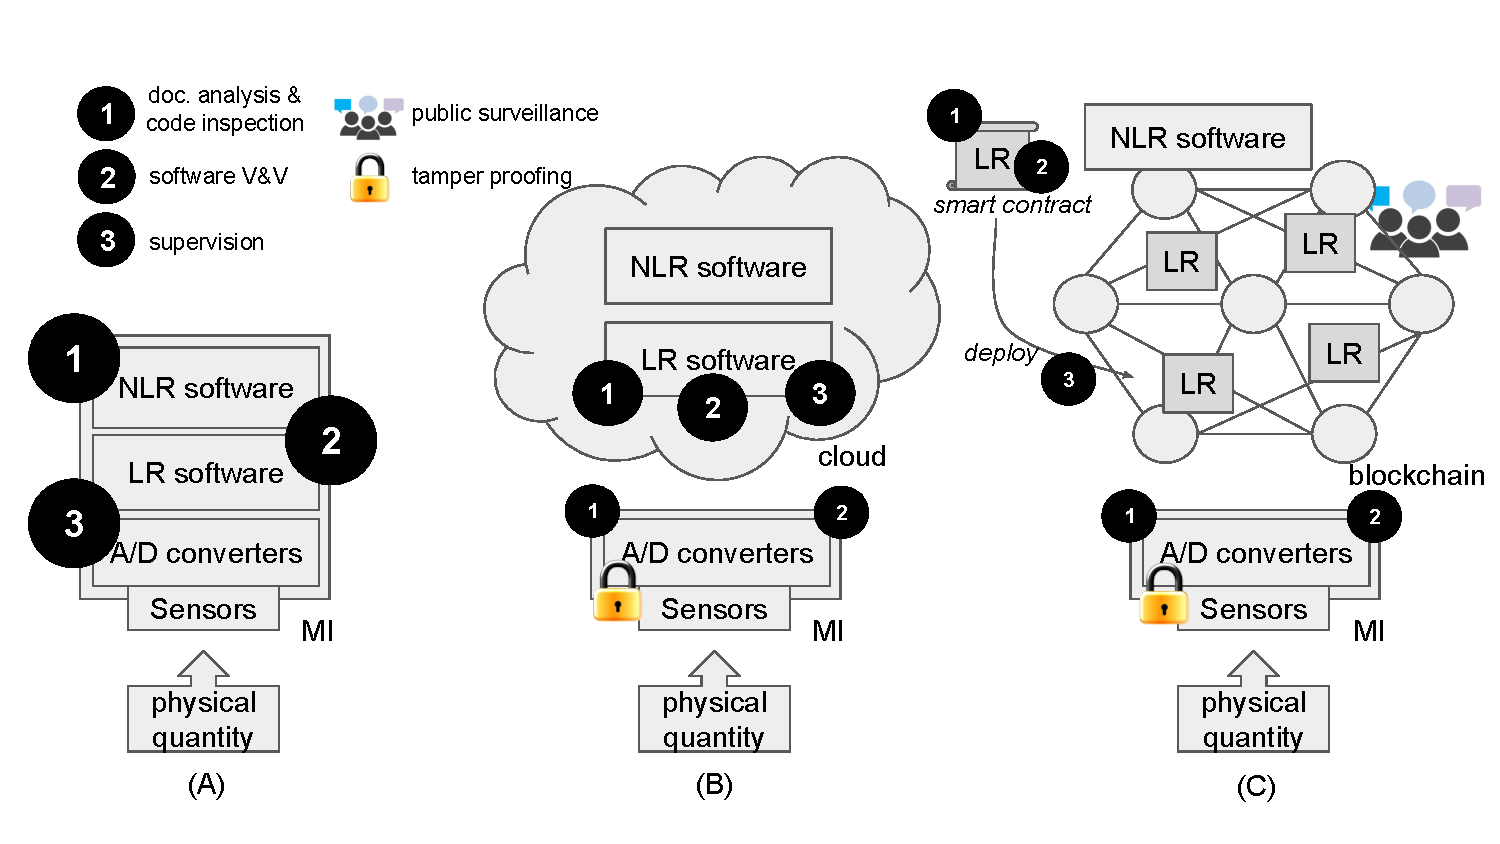
\includegraphics[width=.73\textwidth]{measuring} %[width=2.5in]
\caption{Comparing measuring models: (A) Traditional MI; (B) Cloud Measuring System; (C) Blockchain Measurement System}
\label{f:compare}
\end{figure*}

\subsection{Traditional MI}
\label{s:mi_traditional}
Traditional MI can be seen as dedicated computers calculating measurements of a physical quantity (e.g., size, weight, speed). They include sensors for interfacing with the physical world and AD converters for gathering data, besides other LR and NLR components, which are usually software modules. Sensors and AD converters are also LR components, being usually immutable hardware components (Figure~\ref{f:compare}-A).

Although LR and NLR software separation is a well-known concept, many MI manufacturers do not adopt such practice. The claimed reasons are costs, computational resources restrictions or the existence of a legacy software. As a paradox, despite their complexity, traditional MI software modules are usually monolithic systems. That affects metrological assurance activities substantially, making MI regulation and control more expensive and complex, due to the follow aspects:
\begin{itemize}
\item Type approval can demand MI hardware and software evaluation and checking against a set of reliability requirements. Once LR and NLR are usually tightly coupled, notified bodies leading type approval need to evaluate and attest th compliance of all software modules. In some cases, LR software source code must be inspected for assuring their correctness.
\item Software validation and verification can become more difficult due to the diversity of MI use cases, being many of them hard to reproduce out of the real measurement environment. 
\item Metrological supervision requires that notified bodies have sufficient staff to proceed with MI surveillance activities in both manufacturing and field. Albeit physical seals can be helpful to protect physical components, they are innocuous to protect software components.
%For instance, fuel pumps supervision requires technicians able to inspect electronics components and identify the ones that do not belong to the original design. Software introspection \cite{Boccardo2014} and platform attestation \cite{Peters2015} are approaches used for providing software identification and integrity check.
\end{itemize}

Due to their complexity, the activities also demand a highly qualified professional profile, complementary checking and greater supervision staff proficiency. These factors contribute to make MI regulation and control a very expensive and time consuming process.

\subsection{Cloud-based Measuring System}
\label{s:mi_cloud}
When LR and NLR components are properly separated in independent modules, one could run these modules in different hardware sets connected by well-defined interfaces. Such architecture leads to a \emph{distributed measuring system}. For evaluating its properties, we take a cloud computing MI model inspired in \cite{Oppermann2016}. In this model, LR and NLR software are running as cloud services, outside of MI physical set (Figure~\ref{f:compare}-B). We assume MI communicates with the cloud services using a secure channel (e.g., TLS, HTTPS) and that side channel attacks are infeasible.

When traditional and cloud models are compared, one can observe that the distributed architecture simplifies MI devices. MI practically do not include software components anymore once both LR and NLR software modules are running in the cloud. In practice, MI is now set up as a blend of sensors, AD converters and a communication interface that ables MI to send sensing raw data to the cloud measuring system. Basically, the MI could be designed only based on hardware components (e.g., smart sensors, cryptographic chips), although one should consider that some elementary software could be necessary. In any case, a significantly amount of software is moved to the cloud and works as a service. Consequently, LR and NLR software can be scaled accordingly to the demand.

%Despite of the challenges, we believe distributed measuring enables a trade-off among complexity and features in MI projects. In our conception, MI could adopt a minimalistic architecture, being composed only by sensors and analog-to-digital converters. All other features, including measurement computation, can be implemented in a distributed network. At the same time, legal metrology needs decentralized supervision capabilities once the resources dispose by notified bodies are scarce when compared with the number of deployed MI. We believe such goals can be achieved by distributed measuring systems using blockchains.

\begin{table*}[t]
\centering
\caption{Traditional MI, cloud model and blockchain model security analisys summary}
\label{t:sec_analysis}
\begin{tabularx}{1\textwidth}{|@{}c|l|X|X@{}|}
\toprule
                                  & \multicolumn{1}{c|}{\textbf{Traditional MI}} & \multicolumn{1}{c|}{\textbf{Cloud Model}}                                                                             & \multicolumn{1}{c|}{\textbf{Blockchain Model}}                                                               \\ \midrule
\multicolumn{1}{|c|}{\textbf{R1}} & Required                                     & Required (tamper proofing).                                                                                           & Required (tamper proofing).                                                                                  \\ \midrule
\multicolumn{1}{|c|}{\textbf{R2}} & Required                                     & Required only for LR software in the cloud.                                                                           & Unnecessary, LR smart contracts have integrity enforced due to blockchain properties.                        \\ \midrule
\multicolumn{1}{|c|}{\textbf{R3}} & Required                                     & Required only for LR software in the cloud.                                                                           & Unnecessary, LR smart contracts are signed by notified bodies and checked by blockchain peers on deployment. \\ \midrule
\textbf{A1}                       & Necessary                                    & Necessary, but the evaluation of LR software in the cloud is expected to be easier than MI embedded software.         & Necessary, but the evaluation of LR smart contracts is easier than the other models.                         \\ \midrule
\textbf{A2}                       & Necessary                                    & Necessary, but MI use cases is reduced and V\&V tests can be performed without the need of field tests.               & Necessary, but MI use cases is reduced and V\&V tests can be performed without the need of field tests.      \\ \midrule
\textbf{A3}                       & Necessary                                    & Partially necessary, since periodical inspections take place only in data centers where cloud servers are hosted. & Unnecessary, LR smart contracts have integrity enforced due to blockchain properties.                        \\ \bottomrule
\end{tabularx}
\end{table*}

\subsection{Blockchain-based Measuring System}
\label{s:mi_blockchain}
Now we introduce the \emph{blockchain model} (Figure-\ref{f:compare}-C). We consider that MI basically generate and store reliable measurements of physical quantities while managing the interests of different involved parties (e.g., consumption relations). Thus measurements can be seen as \emph{transactions} whose values must be protected against tampering and unintentional changes \cite{Esche2015}. Such aspects make distributed measuring a typical use case for blockchains applications. 

As a first and intuitive insight, we devise a distributed ledger storing reliable measurement transactions which can be checked by any involved party. In addition, the blockchain also would support the execution of LR (and even NLR) software using smart contracts, which process information from sensors and generate a consolidated measurement value. The integrity of measurements and LR software (as smart contracts) is preserved by blockchain implicit properties \cite{Zheng2017}. The ledger accounting enables the management of cumulative consumption transactions, such as energy and gas metering. If a financial blockchain platform is used, it can integrate billing and payment functions. That is an interesting additional resource when compared to the cloud model.

%In light of these models properties, we claim that distributed measuring systems can be built in both blockchain and cloud architectures. However 
There is a crucial difference between blockchain and cloud models: the liability of the distributed services. In most use cases, MI belong to one of the parties interested in the measurement computing result. Energy and fuel are classical examples where MI are owned by the vendors of the goods. In the cloud model, one can expect that the cloud services will also be held by one of the interested parties. On the other hand, the blockchain is a truly decentralized architecture, being held potentially by several parties. Thus it is expected that a blockchain model will require the contribution of different parties interested in the measurement activities, and consequently it need to be idealized following a different philosophy.

In the blockchain model, we devise measuring as \emph{a service offered by someone without any interest in the measured quantity}. This is remarkably distinct to the traditional scenario where a vendor provides MI for measuring and is rewarded proportionally to the measurement. This idea fits perfectly in the blockchain architecture. Smart contracts can be used for computing measurements based on sensing information. However they are coded by different parties that do not have conflicts of interests related to the measured quantity. Whatever the measurement result, these parties shall be rewarded by a fixed value. That motivates new players to compete by more efficient measuring algorithms once as faster they execute, more credits they earn. Additionally, such strategy creates incentives for keeping the blockchain network since that becomes profitable. One could say that such concept is an innovative idea once it breaks with the manner how MI are traditionally used in consumer relations. Furthermore, it creates a new market for players who want to offer computing services for measuring. 

The blockchain model also enables a set of complementary activities involving MI market and field surveillance that can be done by checking measurements inserted in the distributed ledger. Besides notified bodies, any entity representing society interests, consumers, goods providers, among others, can take part in additional supervision activities. We call that \emph{public surveillance}. Such efforts can include smart contracts for generating redundant measurements for counter-proofing, or statistical analyses against the ledger looking for fraud evidence or patterns, for instance.

%at Section \ref{s:sec_analysis}.

%However, that is not the only advantage. We believe that three main aspects must be emphasize when all the scope of measuring and MI legal control are considered:

% MI can be seen as dedicated computers which calculate measures of a physical quantity (e.g., size, weight, speed). The MI reliability depends on the integrity of measure values, that means the measurement. A measurement is always an approximation of the real physical quantity, being always subject to an error, called uncertain. For each different classes of MI, legal metrology determines an uncertain threshold, which defines the MI precision.

% A measurement can be seen as a transaction. Such analogy is very intuitive in commercial transactions where goods prices are calculated using a MI (e.g., energy meters, fuel pumps, and scales). Attacks against MI usually try to compromise their precision, aiming to economic advantages (e.g, in commercial transactions where price is defined by weight, the seller wishes the scale points a higher measurement, while the buyer wishes the scale registers a lower measurement).

% Based on the aforementioned aspects, we can propose a conceptual model where MI are deployed in a blockchain architecture. MI are devices that generate transactions. Essentially, these transactions records a measurement involving one or more parties. Transactions will be sent to a distributed ledger and, once there, they can not be changed anymore. More than that, we assume that the follow aspects will be fulfilled: distributed measurement, separation of measured quantity and measurement service, and decentralized surveillance. We explain each one of them in details hereafter.

%Considering that, we propose a conceptual model where MI are deployed in a blockchain architecture. MI are devices that generate transactions. Essentially, these transactions records a measurement involving one or more parties. Transactions will be sent to a distributed ledger and, once there, they can not be changed anymore. Furthermore, we assume the following aspects will be fulfilled: %distributed measurement and decentralized surveillance. We explain each one of them hereafter.

% \subsection{Measured quantity \textit{versus} measurement service}
% In trading applications, MI usually belong to one of the involved parties. Energy and fuel are classical examples where MI are owned by the good vendors. Sometimes consumers also have physical access to the MI (e.g., smart meters are deployed at consumers house). Even when MI are properly protected, with sensitive features accessible only by manufacturers or supervision agents, MI ownership represents a security risk once it can motivate attacks and make them easier. A reasonable level of security can be obtained when distributed measurement is implemented. However, traditional approaches using cloud services keeps the measurement procedures under control of the vendor. 
% 
% A better solution is obtained when measuring is a service offered by someone without any interest in the measured quantity. This is remarkably distinct to the traditional scenario where a vendor provides MI for measuring and is rewarded proportionally to the measurement. One could say that such concept is an innovative idea once it breaks with the manner how MI are used in consumer relations and creates a new market for players who want to offer computing services for measurement.
% 
% The described model fits perfectly in blockchain architecture. Such implementation can result from the use of smart contracts for computing measurement based on information from sensors, just like described in the previous section. However the difference is that smart contracts are coded by different parties that do not have conflicts of interests related to the measured quantity. Whatever the measurement result, these parties are going to be rewarded by a fixed value. That motivates new players to compete by more efficient measurement algorithms once faster they execute, more credits they earn. At same time, such model creates an incentive for keeping the blockchain network since that becomes profitable. Furthermore, type approval is favored again, because it is restrict to the smart contract code inspection.

% The blockchain conceptual model has also an important advantage when compared to other distributed approaches: measuring services are offered by someone without any interest in the measured quantity. This is remarkably distinct to the traditional scenario where a vendor provides MI and is rewarded proportionally to the measurement. In trading applications, MI usually belong to one of the involved parties (e.g., fuel pumps are owned by fuel vendors). Sometimes consumers also can have physical access to the MI (e.g., smart meters are deployed inside consumers house). MI ownership and access represent a security risk once that can motivate and facilitate attacks. This problem persists in distributed scenarios using cloud computing as measurement procedures usually are running in machines under control of the vendor. However, when using blockchains, smart contracts are coded by different parties that do not have conflicts of interests related to the measured quantity. Whatever the measurement result, these parties are going to be rewarded by fixed values. That motivates new players to compete by more efficient measurement algorithms while, at same time, creating incentives for participating in the blockchain network. Moreover, type approval is favored again, because it is restrict to the smart contract code inspection.

\section{Security analysis}
\label{s:sec_analysis}
In this section, a security analysis is done by comparing the measuring models discussed in the previous section, considering the attacks and the metrological assurance framework BMAF previously described. We demonstrate how BMAF requirements and activities are impacted when applied on traditional MI and distributed measuring systems. The security analysis is summarized at Table \ref{t:sec_analysis}.

Initially we evaluate the traditional MI security. In this scenario, one should note that BMAF requirements and activities are  necessary to prevent attacks. As already discussed at Section \ref{s:mi_traditional}, the efforts required for proceeding with traditional MI control and supervision activities are distinguished. Type approval and software validation and verification need to comprise all components and software modules. In turn, supervision also requires experienced surveillance technicians to implement inspection and software integrity checks.

When the cloud model is analyzed, one notes that MI become simpler because LR and NLR software are now running in the cloud. At same time, that reduces capabilities of a typical attacker (e.g., consumers do not have physical access to MI software interfaces anymore). The BMAF protection requirements are still necessary, however R2 and R3 requirements are applied on LR software cloud implementation. Supervision activities are also impacted, requiring less efforts to be executed. In A1, the type approval of LR software running in the cloud is expected to require less efforts than embedded software evaluation. Activity A2 is also made simpler once tests can now be performed using interface stubs, without the need of real MI physical environment. In turn, A3 also becomes less expensive because LR software identification and integrity check are executed against cloud servers which are far fewer in number than deployed MI. Finally, field surveillance for checking MI physical seals can also be eliminated. If we assume simplified MI as immutable instruments, they can be conceived as tamper proofing devices. That approach could eliminate the need for verifying MI seals as it implies that the MI will be permanently damaged and any attack trying to explore such vulnerability will not succeed.

Lastly, we evaluate the blockchain model. In addition to presenting the same characteristics of the cloud model, the blockchain security properties also affect BMAF requirements and activities. LR software is now a smart contract whose the deployment rules can be enforced for requiring developers and notified bodies attestation, something that automatically satisfies R3 and makes its regulation unnecessary. Once deployed, LR software is distributed among the network peers and it can not be changed anymore. Blockchain peers can not execute a different smart contract code otherwise blockchain security assumptions will be violated. In consequence, R2 also becomes unnecessary. In terms of activities, although A1 and A2 are still necessary, they should became much simpler when compared to the required effort in the other models. That is because the structure of smart contracts limits significantly the complexity resulting from having different technologies, software components and programming languages, while imposing software separation. Finally, A3 becomes unnecessary in a blockchain network due to the same reasons as R2.

We conclude that while distributed measuring already reduces attackers capabilities, such reduction is more accentuated in the blockchain model. Once LR software is produced by players which are exempted from conflict of interests, many activities related to assure software correctness and integrity are made simpler of even unnecessary. The blockchain security properties plays an important role in this context. 

\section{Challenges Ahead}
Despite blockchains-based measuring systems being a promising approach, there are some challenges that need to be addressed for their use. The main ones as discussed as follow:
%are related to the amount of data expected in some measurement applications, privacy concerns and authentication of external information providers.

\textbf{$\bullet$ The measurement Big Data:} MI usually manipulate a high amount of data. In a large scale scenario (e.g., energy meters in a smart grid), MI can update their measurements faster, generating lots of transactions. A network connecting millions of meters may generate a transaction load unfeasible to be processed by existing blockchains implementations. Benchmark tests in Sousa et al. \cite{Sousa2017} indicate that the best available blockchain platforms are able to reach a peak around of 2000 transactions/second. Such performance is certainly not enough to meet the demand for measurements on a smart grid, for instance. As a possible solution, aggregated measurements can be used for reducing transactions in a blockchain implementation. Smarter MI can also be tried for determining transactions on demand. Another idea is to use \emph{transaction endorsers}, a concept introduced by HyperLedger Fabric \cite{Vukolic2017a,Sousa2017}. Endorsers can execute complex measuring computing, leaving only validation tasks for regular peers.

\textbf{$\bullet$ Measuring and privacy:} Measurements assigned to a specific person allow to infer information about her habits and lifestyle. In a blockchain with public ledger, this problem becomes more serious. One needs to establish an acceptable trade-off between privacy and efficiency. Depending on the application scenario, privacy can require more sophisticated mechanisms for protecting or obfuscating identities, such as pseudonyms or identity protection layers. Permissioned blockchains can also constitute a suitable alternative once they contemplate an access control layer built into blockchain nodes \cite{Vukolic2017a,Vukolic2016}. Access policies can be constrained in such a manner that they satisfy privacy rules and restrictions.
%Blockchains architectures also have evolved to support privacy requirements. Hyperledger 

\textbf{$\bullet$ Communication issues:} Although we consider MI as connected devices, communication can be a problem in applications demanding real-time decisions. That is a restriction for any distributed measuring system over asynchronous networks. Thus blockchain-based measuring is not proper for all MI applications. Furthermore, attacks aiming communication (e.g., DDoS) represent an additional risk, although fully distributed systems as blockchains are more resilient to such attacks than conventional cloud architectures.

\textbf{$\bullet$ Oracles authentication:} External information providers are usually called \emph{oracles} in blockchain architectures. In the described model, MI sensors can be seen as oracles since they are responsible for providing information from the physical world. Despite the fact that sensors are small components which can be protected using physical seals, sensors authentication can be necessary to assure measuring reliability.


\section{Conclusion}
In this paper we discussed how blockchains can be used to support distributed measuring systems. Due to their intrinsic security properties, blockchains can improve MI metrological assurance by imposing restrictions against potential attacks while reducing technical efforts related to regulation and control activities. Despite its promising application, blockchains pose several challenges that need to be faced. The main are related to the amount of data, privacy and oracles authentication. Future works shall bring experimental results and technical strategies for addressing and providing solutions for such difficulties.

% conference papers do not normally have an appendix

% use section* for acknowledgment
\section*{Acknowledgment}
This work was partially sponsored by XXXXX XXXX XXXXX XXXX XXXXX XXXX XXXXX XXXX, grant NNN.NNN/NN-N, by XX XXX XXXX through project XX XX XXX XX.
%This work was partially sponsored by Coordination for the Improvement of Higher Education Personnel (CAPES), grant 99999.008512/2014-0, by FCT through project LaSIGE\\ (UID/CEC/00408/2013).


% \subsection{The measuring Big Data}
% MI applied to massive measuring usually manipulate a big amount of data. For instance, consider a smart meter which basically integrates sensing data of voltage and electrical current sampled in high frequency to calculate energy power. In a high consume scenario, the meter updates its measurements each second, which means more than 80 thousand measurements/day. In a distributed measurement architecture using blockchains, the meter will generate a lot of transactions. When we consider a network integrating 50 million of smart meters, we have the \emph{measuring Big Data} problem and implementations using blockchains become unfeasible.
% 
% Different strategies can be explored to deal with this problem. Aggregated energy measuring already constitutes a practice used for protecting data privacy in measurements and also can be used to reduce the number of transactions in a blockchain implementation. Smarter MI can also be proposed for determining transactions on demand, when the consume exceeds an acceptable threshold. Another resource that should be investigated is the idea of \emph{transactions endorsers}, introduced by HyperLedger Fabric \cite{Vukolic2017a}. Endorsers can be used to execute the measuring complex computing, leaving to smart contracts only the task of validate the measurement.
% 
% \subsection{Measuring and privacy}
% Privacy is a constant challenge in legal metrology. Measurements assigned to a specific person allow to infer various information about her actions and habits. In a blockchain with public ledger, this problem takes on greater proportions.
% 
% The solution here is establish an acceptable trade-off among privacy and efficiency. Depending on the application scenario, privacy can require more sophisticated mechanisms for protecting or obfuscating the identity of the parties involved in the transaction. Permissioned blockchains \cite{Vukolic2017a} can constitute a suitable alternative once they contemplate an access control layer built into blockchain nodes. Access policies can be constrained such a manner they satisfies privacy rules and restrictions.
% %Blockchains architectures also have evolved to support privacy requirements. Hyperledger 
% 
% \subsection{Oracles authentication}
% External information providers are usually called oracles in blockchain architectures. In the described model, MI sensors can be seen as oracles since they are responsible for providing information from physical world. Despite sensors are small components in MI and can be protected using physical seals, sensors authentication can be necessary for assuring measuring reliability.


% An example of a floating figure using the graphicx package.
% Note that \label must occur AFTER (or within) \caption.
% For figures, \caption should occur after the \includegraphics.
% Note that IEEEtran v1.7 and later has special internal code that
% is designed to preserve the operation of \label within \caption
% even when the captionsoff option is in effect. However, because
% of issues like this, it may be the safest practice to put all your
% \label just after \caption rather than within \caption{}.
%
% Reminder: the "draftcls" or "draftclsnofoot", not "draft", class
% option should be used if it is desired that the figures are to be
% displayed while in draft mode.
%
%\begin{figure}[!t]
%\centering
%\includegraphics[width=2.5in]{myfigure}
% where an .eps filename suffix will be assumed under latex, 
% and a .pdf suffix will be assumed for pdflatex; or what has been declared
% via \DeclareGraphicsExtensions.
%\caption{Simulation results for the network.}
%\label{fig_sim}
%\end{figure}

% Note that the IEEE typically puts floats only at the top, even when this
% results in a large percentage of a column being occupied by floats.


% An example of a double column floating figure using two subfigures.
% (The subfig.sty package must be loaded for this to work.)
% The subfigure \label commands are set within each subfloat command,
% and the \label for the overall figure must come after \caption.
% \hfil is used as a separator to get equal spacing.
% Watch out that the combined width of all the subfigures on a 
% line do not exceed the text width or a line break will occur.
%
%\begin{figure*}[!t]
%\centering
%\subfloat[Case I]{\includegraphics[width=2.5in]{box}%
%\label{fig_first_case}}
%\hfil
%\subfloat[Case II]{\includegraphics[width=2.5in]{box}%
%\label{fig_second_case}}
%\caption{Simulation results for the network.}
%\label{fig_sim}
%\end{figure*}
%
% Note that often IEEE papers with subfigures do not employ subfigure
% captions (using the optional argument to \subfloat[]), but instead will
% reference/describe all of them (a), (b), etc., within the main caption.
% Be aware that for subfig.sty to generate the (a), (b), etc., subfigure
% labels, the optional argument to \subfloat must be present. If a
% subcaption is not desired, just leave its contents blank,
% e.g., \subfloat[].


% An example of a floating table. Note that, for IEEE style tables, the
% \caption command should come BEFORE the table and, given that table
% captions serve much like titles, are usually capitalized except for words
% such as a, an, and, as, at, but, by, for, in, nor, of, on, or, the, to
% and up, which are usually not capitalized unless they are the first or
% last word of the caption. Table text will default to \footnotesize as
% the IEEE normally uses this smaller font for tables.
% The \label must come after \caption as always.
%
%\begin{table}[!t]
%% increase table row spacing, adjust to taste
%\renewcommand{\arraystretch}{1.3}
% if using array.sty, it might be a good idea to tweak the value of
% \extrarowheight as needed to properly center the text within the cells
%\caption{An Example of a Table}
%\label{table_example}
%\centering
%% Some packages, such as MDW tools, offer better commands for making tables
%% than the plain LaTeX2e tabular which is used here.
%\begin{tabular}{|c||c|}
%\hline
%One & Two\\
%\hline
%Three & Four\\
%\hline
%\end{tabular}
%\end{table}


% Note that the IEEE does not put floats in the very first column
% - or typically anywhere on the first page for that matter. Also,
% in-text middle ("here") positioning is typically not used, but it
% is allowed and encouraged for Computer Society conferences (but
% not Computer Society journals). Most IEEE journals/conferences use
% top floats exclusively. 
% Note that, LaTeX2e, unlike IEEE journals/conferences, places
% footnotes above bottom floats. This can be corrected via the
% \fnbelowfloat command of the stfloats package.

% trigger a \newpage just before the given reference
% number - used to balance the columns on the last page
% adjust value as needed - may need to be readjusted if
% the document is modified later
%\IEEEtriggeratref{8}
% The "triggered" command can be changed if desired:
%\IEEEtriggercmd{\enlargethispage{-5in}}

% references section

% can use a bibliography generated by BibTeX as a .bbl file
% BibTeX documentation can be easily obtained at:
% http://mirror.ctan.org/biblio/bibtex/contrib/doc/
% The IEEEtran BibTeX style support page is at:
% http://www.michaelshell.org/tex/ieeetran/bibtex/
\bibliographystyle{IEEEtran}
% argument is your BibTeX string definitions and bibliography database(s)
\bibliography{IEEEabrv,mythesis}
%
% <OR> manually copy in the resultant .bbl file
% set second argument of \begin to the number of references
% (used to reserve space for the reference number labels box)
% \begin{thebibliography}{1}
% 
% \bibitem{IEEEhowto:kopka}
% H.~Kopka and P.~W. Daly, \emph{A Guide to \LaTeX}, 3rd~ed.\hskip 1em plus
%   0.5em minus 0.4em\relax Harlow, England: Addison-Wesley, 1999.
% 
% \end{thebibliography}

% that's all folks
\end{document}